\documentclass[french]{template}

\begin{document}

\titre{Projet Newtonoid}
\UE{Programmation Fonctionnelle}
\enseignant{Guilaume \textsc{Dupont}}
\eleves{Romain \textsc{Haessler} \\ Benjamin \textsc{Pascal} \\ Leïlie \textsc{Canillac} \\ Vianney \textsc{Hervy}}

\fairemarges
\fairepagedegarde
\tabledematieres

\newpage

\section{Usage}

\begin{itemize}
    \item \textbf{Compilation:} \texttt{dune build}
    \item \textbf{Tests:} \texttt{dune runtest}
    \item \textbf{Exécution (par défaut)\footnote{Il est possible de choisir une configuration de jeu ainsi que des niveaux:\\\texttt{dune exec bin/newtonoid.exe configs/default-dark.conf levels/level-1.txt levels/level-2.txt}}:} \texttt{dune exec bin/newtonoid.exe}
\end{itemize}

Les contrôles sont indiqués dans le jeu directement

\section{Architecture}

Les sources sont réparties en deux répertoires: \texttt{bin} et \texttt{lib}.

\begin{itemize}
    \item \texttt{bin} contient le programme principal \texttt{newtonoid.ml} qui peut utiliser les modules de la bibliothèque \texttt{Libnewtonoid}.
    \item \texttt{lib} contient les modules et interfaces impémentant les divers éléments du jeu. Le fichier \texttt{lib/dune} contient une directive pour créer une bibliothèque appelée \texttt{Libnewtonoid} contenant tous les modules de \texttt{lib}.
\end{itemize}

Les répertoires \texttt{configs} et \texttt{levels} contiennent respectivement des configuration et des niveaux d'exemple.

\subsection{Modules}

La plupart des modules de \texttt{Libnewtonoid} sont dotés d'une interface documentée en \texttt{.mli} et de tests. Certains modules sont relatifs à des objets: \texttt{Ball}, \texttt{Box}, \texttt{Brick}, \texttt{Level}, \texttt{Paddle}, \texttt{State}. Tandis que d'autres sont un groupement de fonctions nécessaires à une fonctionnalité: \texttt{Collision}, \texttt{Input}, \texttt{Iterator}, \texttt{LoadLevel}, \texttt{Utils}, \texttt{ParamValidator}, \texttt{Iterator}.

La plupart des modules contiennent un sous-module foncteur (au sens d'OCaml) paramétré par un module de configuration \texttt{P}. On a donc une structure récurrente de la forme: \texttt{module Make(P: Params)} qui permet d'instancier le foncteur avec les paramètres fournis par l'utilisateur.

\section{Objets}

Chaque objet du jeu est modélisé par un type enregistrement afin de permettre un accès efficace aux différents champs (par opposition aux tuples qui nécessitent du filtrage par motif). Chaque type objet est appelé \texttt{t} et est défini dans son propre module qui regroupe les fonctions associées. Parmis celles-ci, on note surtout \texttt{make}, \texttt{draw} et \texttt{draw\_shadow} et qui permettent respectivement de créer un objet, de l'afficher à l'écran et de dessiner son ombre.

Les objets définis juste après sont mieux documentés dans leur interface \texttt{.mli}.
\begin{itemize}
    \item \textbf{Ball:} la balle du jeu, rebondit avec un facteur d'accélération soumise à la gravité.
    \item \textbf{Box:} Le rectangle de jeu, propre à chaque niveau.
    \item \textbf{Brick:} Les briques du jeu, avec un type de brique (\texttt{Standard}, \texttt{Unbreakable} etc) et un nombre de pv, une couleur, etc associés.
    \item \textbf{Paddle:} La raquette du joueur, se déplace horizontalement. Sa vitesse horizontale est calculée à chaque frame en fonction de sa position précédente.
\end{itemize}

\subsection{États de jeu}

Nous avons décidé de n'utiliser qu'un seul flux d'état de premier élément l'état initial et de fonction de "génération" \texttt{STATE.update}. C'est une sorte d'\texttt{unfold}\footnote{voir \texttt{Utils.unfold2}} qui génère ce flux. Ainsi, à partir de l'état initial et du flux de la souris, on obtient le flux des états de jeu. Un \texttt{STATE.t} est un enregistrement contenant les différents objets du jeu (le score, état de la balle, de la raquette, du niveau, etc). Son \texttt{game\_status} est un type somme qui contient le status de l'état actuel (en pause, en jeu, fini etc). La figure \ref{fig:graph} montre le graphe de transition des états de jeu.

\begin{figure}
    \centering
    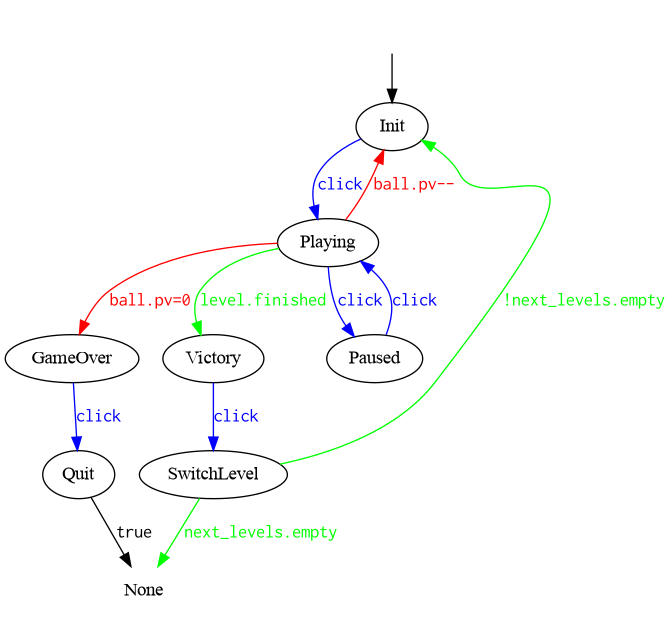
\includegraphics[width=\textwidth]{img/graph.png}
    \caption{Graphe de transition des états de jeu}
    \label{fig:graph}
\end{figure}

\subsection{Niveaux de jeu}

Initialement, un niveau de jeu était défini en OCaml et chaque brique ajoutée séparément. C'était à la fois verbeux et peu pratique. Nous avons donc "développé" une syntaxe très simple pour définir un niveau textuellement. Chaque type de brique est représenté par un caractère différent et l'air est représenté par un espace. Les bordures sont fixées avec les caractères tiret et barre verticale. Deux exemples de niveaux sont donnés à la figure \ref{fig:level.txt}.

Des exemples de niveaux sont disponibles dans le répertoires \texttt{levels}.

Cette solution a donné une liberté de création qui pose un autre problème. Désormais, les niveaux peuvent avoir différents formats. Afin d'éviter les niveaux débordant de la fenêtre, les dimensiosn de cette dernière sont fonction directe des dimensions du niveau et de la taille des briques.

\begin{figure}
    \begin{minipage}{0.4\textwidth}
        \begin{verbatim}
        |----------------|
        | ############## |
        | ============== |
        | ++++++++++++++ |
        |                |
        |                |
        |                |
        |----------------|
        \end{verbatim}
    \end{minipage}
    \hfill
    \begin{minipage}{0.4\textwidth}
        \begin{verbatim}
        |----------------|
        | @+ + + + + + @ |
        | @ + + + + + +@ |
        | @+ + + + + + @ |
        | @ + + + + + +@ |
        | @@@@@@@@@@@@@@ |
        |                |
        |----------------|
        \end{verbatim}
    \end{minipage}
    \caption{Exemples de niveau}
    \label{fig:level.txt}
\end{figure}

\section{Paramètres}

Nous avons vite compris que la possibilité de changer efficacement les paramètres était cruciale pour le développement et pratique pour le joueur. C'est pourquoi nous avons créé un module \texttt{Params} qui contient tous les paramètres du jeu. L'idée était de paramétrer les autres modules en fonction de \texttt{Params}. Ainsi, chaque module est en partie défini par les paramètres qui lui sont donnés.

Cette paramétrisation des modules permet de diminuer le nombre d'arguments des fonctions ainsi que la présene de valeurs "magiques" dans le code.

Pour faciliter la gestion des paramètres, nous avons développé un "parsing" primitif de fichier en \texttt{.conf} qui récupère les paramètres du jeu et crée un module \texttt{Params} correspondant. Cette fonctionnalité est implémentée via le foncteur (au sens d'OCaml) \texttt{Params.Make} qui prend en argument un simple module contenant le nom du fichier de configuration et renvoie un module \texttt{Params}.

Des exemples de fichiers de configuration sont disponibles dans le répertoire \texttt{configs}.

\section{Tests}

Les tests unitaires de ce projet sont réalisés avec la bibliothèque \texttt{ppx\_inline\_test}. Leur code se trouve dans le répertoire \texttt{test}. Les tests sont lancés avec la commande \texttt{dune runtest}.

Afin d'éviter des paramétrages insensés, à chaque lancement de jeu, \texttt{paramValidator.ml} valide (ou non) les valeurs données par l'utilisateur dans le fichier de configuration. On vérifie par exemple que \texttt{ball\_r > 0}, \texttt{ball\_init\_vy <= ball\_max\_vy} etc.

\section{Améliorations et manquements}

\begin{itemize}
    \item \textbf{Gestion de l'espace de jeu:} À chaque frame, on vérifie les collision balle/brique pour toutes les briques. Le développement d'un quadtree (voir \texttt{lib/quadtree.\{ml,mli\}}) n'a pas abouti pour cause de blocage lors de la gestion des briques chevauchant plusieurs cadrans. Toutefois, le jeu tourne bien sans cette optimisation même avec un grand nombre de briques.
    \item \textbf{Sauvegarde:} Il serait intéressant de pouvoir sauvegarder et charger une partie en cours.
    \item \textbf{Niveaux:} La création de niveaux plus complexes et la gestion de niveaux aléatoires.
    \item \textbf{Effets:} Ajouter des effets spéciaux (briques qui explosent, balle qui se divise, etc).
    \item \textbf{Son:} Ajouter des effets sonores.
    \item \textbf{Lore:} Ajouter une histoire au jeu.
\end{itemize}

\end{document}